%!TEX root = /Users/ede/Documents/Master/19_AS/Ausarbeitung/as-ausarbeitung.tex
\section{Tag-Ranking Verfahren} % (fold)
\label{sec:tag_ranking_verfahren}
Hier erfolgt die Darstellung der Tag-Ranking Verfahren im genauen.

% 
% 
% \begin{itemize}
%   \item   Visual diversification of image search results \cite{diversification}
%   \item   Tag ranking \cite{ranking}
%   \item   Learning to tag \cite{learningToTag}
%   \item   Learning tag relevance by neighbor voting for social image retrieval \cite{learningtagrelevance}
%   \item   Improving recommendation lists through topic diversification \cite{improvingRecommendations}
%   \item   Why we tag: motivations for annotation in mobile and online media \cite{whyWeTag}
%   \item   Flickr tag recommendation based on collective knowledge \cite{collectiveKnowledge}
% \end{itemize}

\subsection{Ranking basierend auf kollektivem Wissen nach Sigurbjörnsson und van Zwol} % (fold)
\label{sub:ranking_basierend_auf_kollektivem_wissen_nach_zwol}




\begin{itemize}
  \item Tag co-occurrence is the key to our tag recommendation approach, and only works reliable when a large quantity of supporting data is available.
  \item We define the co-occurrence between two tags to be the number of photos [in our collection] where both tags are used in the same annotation.
  \item Symmetric measures vs. Asymmetric measures
  \item Zweiter Schritt: Tag Aggregation and Promotion
  \begin{itemize}
    \item Aggregation durch \emph{Vote} und \emph{Sum} Verfahren
    \item Priorisierung der Tags durch \emph{Stability-promotion} und \emph{Descriptiveness-promotion}
  \end{itemize}
\end{itemize}

\begin{figure}[htbp]
  \centering
    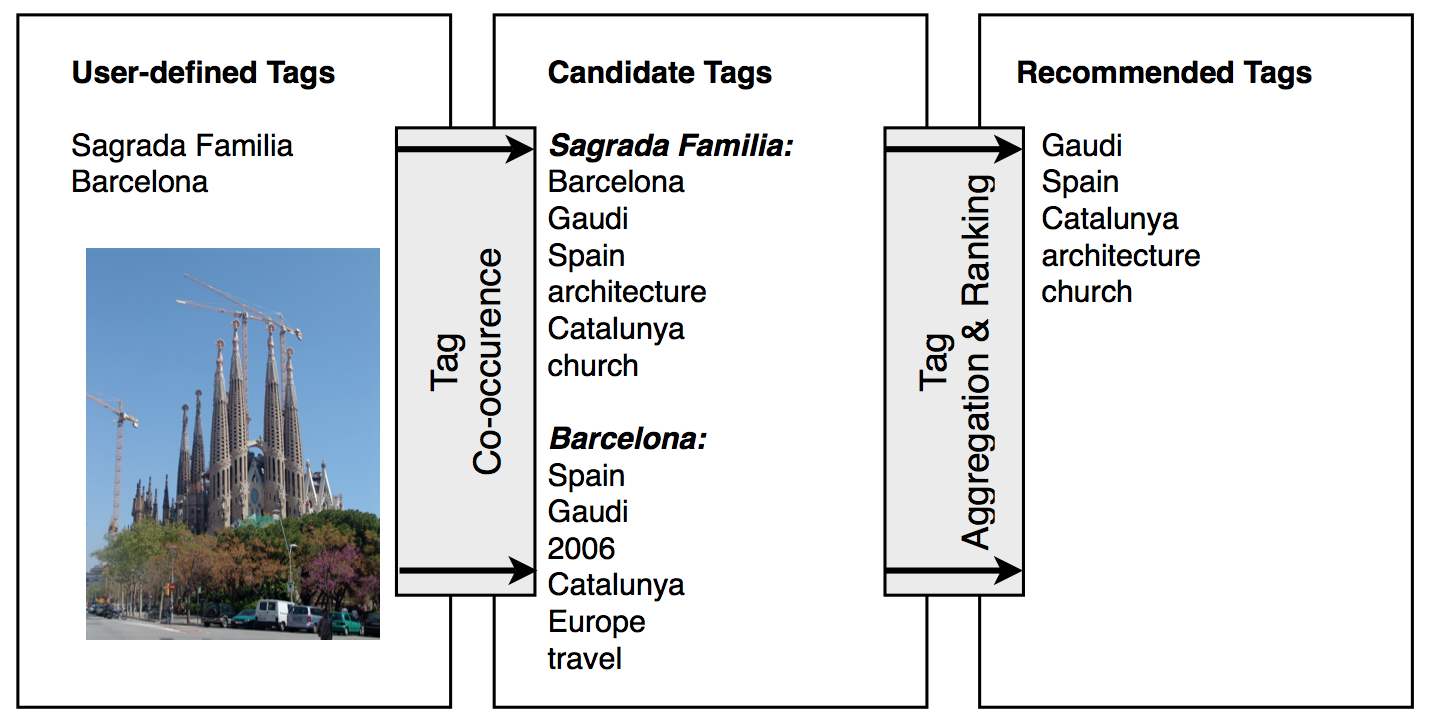
\includegraphics[height=3in]{images/collective_knowledge_system_overview.png}
  \caption{System overview of the tag recommendation process aus \cite{collectiveKnowledge}}
  \label{fig:images_collective_knowledge_system_overview}
\end{figure}

 - Verfahren basiert auf Tag co-occurrence
Tag co-occurrence is the key to our tag recommendation approach, and only works reliable when a large quantity of supporting data is available.

 - Definition von co-occurrence nach \cite{collectiveKnowledge}
   - sehr einfache basis für verfahren
 - um die den wert der co-occurrence von der allgemeinen verwendungs-frequenz zu trennen, wird dieser wert normalisiert. 
 - co-occurrence als asymmetrische Maßeinheit
   - unterschiedliche Normalisierung möglich
   - im gegensatz zu einer symmetrischen normalisierung, die eher die Äquivalenz von zwei tags angibt, da hierbei die summe der anzahl beider tags als divisor verwendet wird und somit die gemeinsame Auftrittswahrscheinlich für diese beiden Tags angegeben wird.
\begin{figure}[hptb]
  \begin{equation}
  \label{symmetricNormalization}
   J(t_i, t_j) := \frac{\vert t_i \cap t_j \vert}{ \vert t_i \cup t_j \vert }
  \end{equation}
\end{figure}
   
   - bei der asymmetrischen normalisierung wird die anzahl des gemeinsamen auftretens durch die anzahl des ersten tags dividiert. damit wird also erfasst, wie oft tag ti gemeinsam mit tj gelistet wird, was beim vorschlagen von tags mehr sinn macht, damit der inhalt der photos möglichst vielfältig anstatt genau getaggt werden kann.
   % TODO: hier gibts kritikmöglichkeit, evtl. später aufgreifen.
\begin{figure}[hptb]
 \begin{equation}
 \label{symmetricNormalization}
  J(t_i \vert t_j) := \frac{\vert t_i \cap t_j \vert}{ \vert t_i \vert }
 \end{equation}
\end{figure}

% subsection ranking_basierend_auf_kollektivem_wissen_nach_zwol (end)

\subsection{Verbesserung der Relevanz von Tags durch einen Random Walk nach Liu u. a.} % (fold)
\label{sub:verbesserung_der_relevanz_durch_einen_random_walk}

\begin{itemize}
  \item Wahrscheinlichkeitsorientierte Schätzung der Relevanz von Tags.
  \item Random-Walk basierte Verfeinerung des Rankings
    
    \begin{itemize}
      \item Aufbau eines Beziehungs-Graphen der Tags.
      \item Random Walk über den Graphen
    \end{itemize}
\end{itemize}

\begin{figure}[htbp]
  \centering
    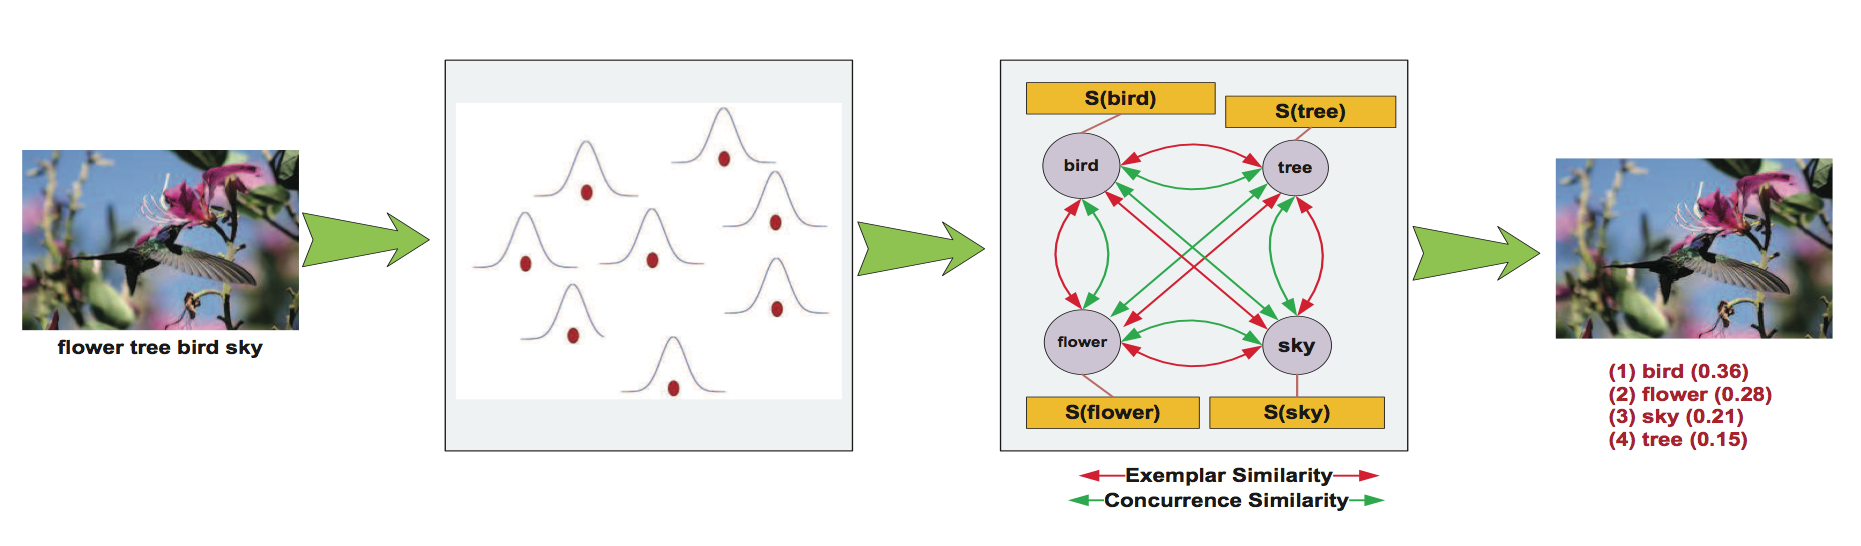
\includegraphics[height=2in]{images/tag_ranking_verfahren.png}
  \caption{The illustrative scheme of the tag ranking approach. A probabilistic method is first adopted to estimate tag relevance score. Then a random walk-based refinement is performed along the tag graph to further boost tag ranking performance aus \cite{ranking}}
  \label{fig:images_tag_ranking_verfahren}
\end{figure}


Ausführliche Beschreibung des Verfahrens folgt.

% subsection verbesserung_der_relevanz_durch_einen_random_walk (end)
% section tag_ranking_verfahren (end)
